\documentclass{article}

% Use the COLM 2026 conference style (submission mode = anonymous)
\usepackage[submission]{colm2026_conference}

% Configure natbib for numbered citations
\setcitestyle{numbers,square}

% Standard packages
\usepackage{times}
\usepackage{graphicx}
\usepackage{amsmath,amsfonts,amssymb}
\usepackage{booktabs}
\usepackage{multirow}
\usepackage{algorithm}
\usepackage{algorithmic}
\usepackage{tikz}
\usepackage{pgfplots}
\pgfplotsset{compat=1.18}
\usetikzlibrary{shapes,arrows,positioning,calc,patterns}

% Math commands
\input{math_commands}

% Hyperref for cross-references (but not visible URLs in submission mode)
\usepackage[hidelinks]{hyperref}

% Title and authors (anonymized for submission)
\title{Agent Memory Below the Prompt: \\
Persistent Q4 KV Cache for Multi-Agent LLM Inference on Edge Devices}

% Anonymous submission
\author{Anonymous Authors}

\begin{document}

\maketitle

\begin{abstract}
Multi-agent LLM workflows on Apple Silicon spend most of their time re-computing attention state. A 5-agent system with 4K tokens each waits 77 seconds after every server restart while each agent re-prefills from scratch. We persist each agent's KV cache to disk in 4-bit quantized format and reload it in under 700\,ms. Three components make this work: (1)~a block pool giving each agent an isolated, persistent Q4 KV cache stored in safetensors, (2)~BatchQuantizedKVCache for concurrent inference over multiple agents' quantized caches, and (3)~cross-phase context injection that lets agents accumulate attention state across conversation phases without re-computation. On Gemma~3 12B and DeepSeek-Coder-V2-Lite 16B at typical deployment lengths (4K context), warm disk reload reduces TTFT from 15.5s to 513\,ms (30$\times$) and from 3.9s to 252\,ms (16$\times$). At 32K context, the speedup reaches 130$\times$ and 74$\times$. Batched serving of two concurrent agents reaches 22.4 and 64.8 system tokens/second with warm cache. The system handles both dense GQA (Gemma) and MoE MLA (DeepSeek) architectures through a model-agnostic abstraction. In multi-agent workflows, a 10-expert routing benchmark shows 24$\times$ TTFT reduction when querying cached experts. Open-source at \texttt{[anonymized]}.
\end{abstract}

\section{Introduction}
\label{sec:intro}

Five agents, each holding 4,096 tokens of conversation history. The server restarts. On an Apple M4~Pro, each agent needs 15.5 seconds to re-prefill its context through the model. Total: 77 seconds of dead time before any agent can respond.

This is the cold-start problem for multi-agent LLM inference on edge devices. Datacenter GPUs process tokens at 10,000+/second, making a 4K re-prefill a 400\,ms annoyance. Apple Silicon processes them at roughly 260/second (Gemma~3 12B, M4~Pro). The gap is 40$\times$.

We eliminate re-prefill by persisting each agent's KV cache. The cache produced during prefill is the agent's memory at the attention layer. Instead of discarding it after each request (as vLLM~\cite{kwon2023pagedattention} and SGLang~\cite{zheng2024sglang} do) or holding it only in volatile RAM, we write it to disk in 4-bit quantized format and reload it when the agent resumes. Context restoration drops from 15.5 seconds to 513\,ms (warm, disk) or 709\,ms (hot, memory) at 4K context on Gemma~3 12B.

This differs from retrieval-augmented generation (RAG). RAG stores text chunks in vector databases and re-runs prefill over retrieved text on every request~\cite{sarthi2024raptor}. We store the computed attention state itself. RAG costs O(n) per request. Cache reload costs O(1).

\paragraph{Contributions.} (1)~A persistent block pool giving each agent isolated, quantized KV cache surviving server restarts and device reboots, stored in safetensors format. (2)~BatchQuantizedKVCache for concurrent Q4 inference over multiple agents' caches, with an interleaved prefill+decode scheduler. (3)~Cross-phase context injection treating KV cache as working memory, letting agents accumulate attention state across conversation phases without re-computation. (4)~Evaluation across two architecturally distinct models, dense GQA (Gemma~3 12B) and MoE MLA (DeepSeek-Coder-V2-Lite 16B), showing the abstraction generalizes.

\section{Background}
\label{sec:background}

\subsection{Re-Prefill Costs on Edge Hardware}

LLM inference has two phases: prefill (process all input tokens in parallel, producing KV pairs for each attention layer) and decode (generate output tokens one at a time, attending to cached KV state). Prefill is compute-bound. Decode is memory-bandwidth-bound.

On Apple M4~Pro (24\,GB unified memory, 273\,GB/s bandwidth), we measured cold-start prefill for Gemma~3 12B: 4.0s at 1K tokens, 15.5s at 4K, 32.9s at 8K, 71.1s at 16K, 165.2s at 32K. For a 5-agent workflow where each agent has 4K context, a server restart imposes 77 seconds of re-prefill. DeepSeek-Coder-V2-Lite is faster per token (1.1s at 1K, 3.9s at 4K) but the problem scales identically.

\subsection{Unified Memory Architecture}

% Figure 4: UMA vs Discrete Memory Architecture
% TikZ diagram showing zero-copy vs PCIe bottleneck

\begin{figure}[t]
\centering
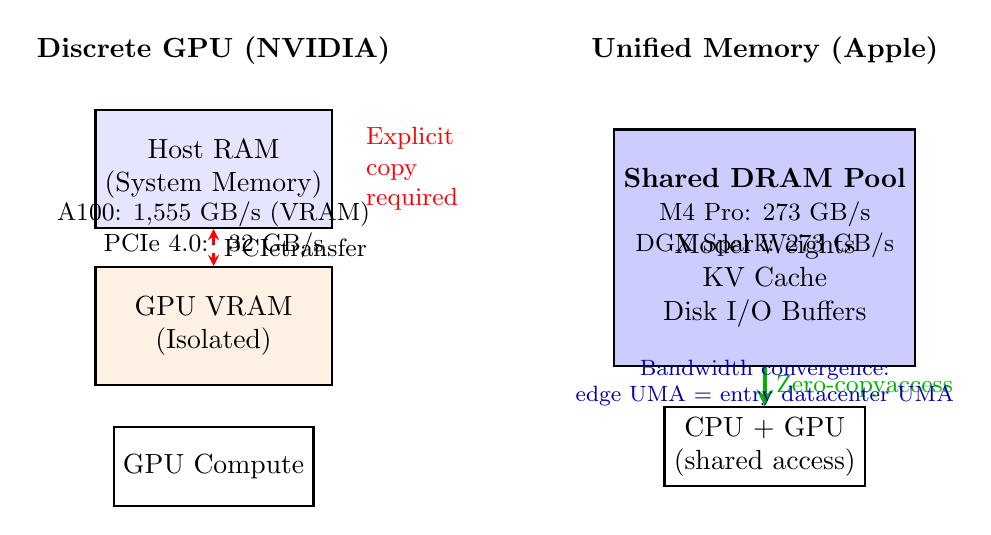
\begin{tikzpicture}[
    node distance=0.8cm,
    component/.style={rectangle, draw=black, thick, minimum width=2.5cm, minimum height=1cm, align=center},
    memory/.style={rectangle, draw=black, thick, fill=blue!10, minimum width=3cm, minimum height=1.5cm, align=center},
    arrow/.style={->, >=stealth, thick},
    zerocopy/.style={->, >=stealth, ultra thick, draw=green!70!black},
    pcie/.style={<->, >=stealth, thick, draw=red, dashed}
]

% Left side: Discrete GPU (NVIDIA)
\node[font=\bfseries] (discrete_title) at (0,3.5) {Discrete GPU (NVIDIA)};

\node[memory] (host_mem) at (0,2) {Host RAM\\(System Memory)};
\node[memory, fill=orange!10] (gpu_mem) at (0,0) {GPU VRAM\\(Isolated)};
\node[component, below=0.5cm of gpu_mem] (gpu_compute) {GPU Compute};

\draw[pcie] (host_mem) -- node[right, font=\small] {PCIe\\transfer} (gpu_mem);
\node[right=0.3cm of host_mem, font=\small, text=red, align=left] {Explicit\\copy\\required};

% Right side: UMA (Apple Silicon)
\node[font=\bfseries] (uma_title) at (7,3.5) {Unified Memory (Apple)};

\node[memory, minimum width=3.5cm, minimum height=3cm, fill=blue!20] (uma_mem) at (7,1) {
    \textbf{Shared DRAM Pool}\\
    ~\\
    Model Weights\\
    KV Cache\\
    Disk I/O Buffers
};

\node[component, below=0.5cm of uma_mem] (cpu_gpu) {CPU + GPU\\(shared access)};

\draw[zerocopy] (uma_mem.south) -- node[right, font=\small, text=green!70!black] {Zero-copy\\access} (cpu_gpu);

% Bandwidth annotations
\node[below=1.5cm of discrete_title, font=\small, align=center] {
    A100: 1,555 GB/s (VRAM)\\
    PCIe 4.0: ~32 GB/s
};

\node[below=1.5cm of uma_title, font=\small, align=center] {
    M4 Pro: 273 GB/s\\
    DGX Spark: 273 GB/s
};

% Convergence note
\node[below=3.5cm of uma_title, font=\footnotesize, text=blue!70!black, align=center] {
    Bandwidth convergence:\\
    edge UMA = entry datacenter UMA
};

\end{tikzpicture}
\caption{Memory architecture comparison. Discrete GPUs isolate model weights in VRAM, requiring explicit PCIe transfers (32 GB/s bottleneck). Unified Memory Architecture (UMA) provides zero-copy access to a shared DRAM pool. M4 Pro and DGX Spark converge at 273 GB/s bandwidth, though datacenter accelerators still dominate compute throughput.}
\label{fig:uma}
\end{figure}


Apple Silicon's Unified Memory Architecture (UMA) shares a single DRAM pool between CPU and GPU without PCIe transfers. The M4~Pro provides 273\,GB/s bandwidth, matching NVIDIA's DGX~Spark workstation (\$3,999, 128\,GB unified)~\cite{nvidia2025dgxspark}. Datacenter accelerators still dominate compute throughput (10--50$\times$ higher prefill speeds), but UMA enables zero-format-conversion paths between model weights, KV cache, and disk I/O buffers: safetensors files are loaded via \texttt{mx.load()} into MLX arrays without intermediate NumPy conversion.

The constraint: 24\,GB total capacity shared by OS, model weights, and KV cache. Gemma~3 12B Q4 weights consume roughly 6.5\,GB, leaving 17.5\,GB for everything else. Q4 KV cache reduces per-layer storage by 72\% compared to FP16, which matters when caching multiple agents' state simultaneously.

\section{System Design}
\label{sec:design}

% Figure 1: System Architecture
% TikZ diagram showing: Agent -> Block Pool -> Q4 Pipeline -> Disk

\begin{figure}[t]
\centering
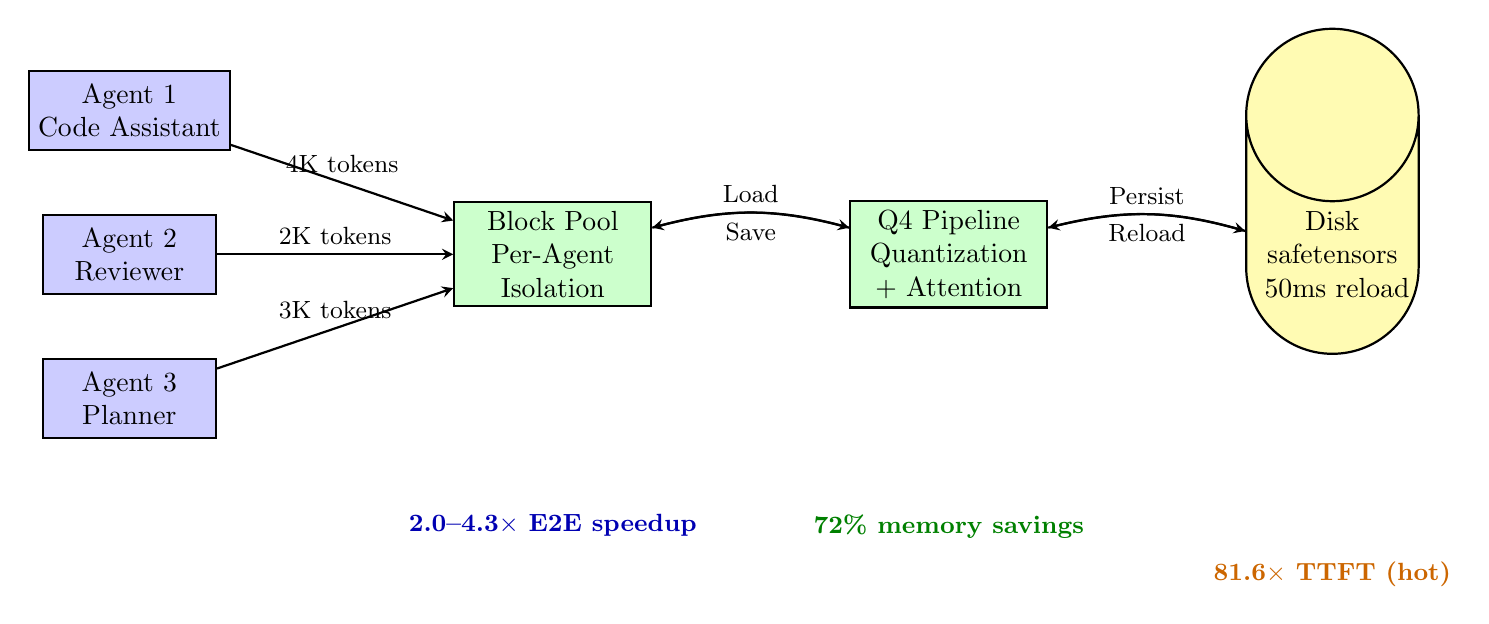
\begin{tikzpicture}[
    node distance=1.5cm and 2cm,
    agent/.style={rectangle, draw=black, thick, fill=blue!20, minimum width=2.2cm, minimum height=1cm, align=center},
    component/.style={rectangle, draw=black, thick, fill=green!20, minimum width=2.5cm, minimum height=1.2cm, align=center},
    storage/.style={cylinder, draw=black, thick, fill=yellow!30, minimum width=2cm, minimum height=1.2cm, align=center, shape border rotate=90},
    arrow/.style={->, >=stealth, thick},
    label/.style={font=\small}
]

% Agents
\node[agent] (a1) {Agent 1\\Code Assistant};
\node[agent, below=0.8cm of a1] (a2) {Agent 2\\Reviewer};
\node[agent, below=0.8cm of a2] (a3) {Agent 3\\Planner};

% Block Pool
\node[component, right=3cm of a2] (bp) {Block Pool\\Per-Agent\\Isolation};

% Q4 Pipeline
\node[component, right=2.5cm of bp] (q4) {Q4 Pipeline\\Quantization\\+ Attention};

% Disk Storage
\node[storage, right=2.5cm of q4] (disk) {Disk\\safetensors\\~50ms reload};

% Arrows from agents to block pool
\draw[arrow] (a1) -- node[above, label] {4K tokens} (bp);
\draw[arrow] (a2) -- node[above, label] {2K tokens} (bp);
\draw[arrow] (a3) -- node[above, label] {3K tokens} (bp);

% Arrow from block pool to Q4 pipeline
\draw[arrow, bend left=15] (bp) to node[above, label] {Load} (q4);
\draw[arrow, bend right=15] (q4) to node[below, label] {Save} (bp);

% Arrow from Q4 pipeline to disk
\draw[arrow, bend left=15] (q4) to node[above, label] {Persist} (disk);
\draw[arrow, bend right=15] (disk) to node[below, label] {Reload} (q4);

% Results annotations
\node[below=2.5cm of bp, align=center, font=\small\bfseries, text=blue!70!black] {2.0--4.3$\times$ E2E speedup};
\node[below=2.5cm of q4, align=center, font=\small\bfseries, text=green!50!black] {72\% memory savings};
\node[below=2.5cm of disk, align=center, font=\small\bfseries, text=orange!80!black] {81.6$\times$ TTFT (hot)};

\end{tikzpicture}
\caption{System architecture. Multiple agents maintain isolated KV caches in a persistent block pool. The Q4 pipeline quantizes cache data on save and operates directly on quantized tensors during attention. Disk persistence enables sub-100ms reload (warm) vs seconds of re-prefill (cold).}
\label{fig:architecture}
\end{figure}


\subsection{Block Pool with Per-Agent Isolation}

The block pool partitions KV cache into fixed-size blocks of 256 tokens, organized by agent ID. Each agent's cache consists of AgentBlocks (a mapping from agent ID to a list of KVBlock instances) where each KVBlock stores per-layer key/value tensors in Q4 format (uint32 packed data + float16 scales/biases). A ModelCacheSpec captures architectural parameters (layer count, KV head count, head dimensions, quantization settings) without model-specific logic.

Each agent's cache is independently addressable. Server restart, model swap, or concurrent inference over multiple agents cannot corrupt or mix cache state. The block pool enforces namespace isolation at the data structure level.

\subsection{Q4 Quantization Pipeline}

KV cache flows through the system in 4-bit quantized format at every stage:

\begin{enumerate}
    \item \textbf{Disk}: uint32 packed weights + float16 scales/biases in safetensors format
    \item \textbf{Memory}: Same format, loaded via memory-mapped I/O
    \item \textbf{Attention}: MLX's \texttt{quantized\_scaled\_dot\_product\_attention()} operates directly on Q4 tensors
\end{enumerate}

For a layer with $h$ KV heads, head dimension $d$, sequence length $n$, and group size $g{=}64$: FP16 stores $2hdn \times 2$ bytes (K+V, 2 bytes each); Q4 stores $2hdn / 2 + 2hd(n/g) \times 2$ bytes (packed uint32 + float16 scales/biases). The ratio $\text{Q4}/\text{FP16} = (0.5 + 4/g) / 2 = 0.281$ for $g{=}64$, yielding 72\% memory reduction per layer regardless of model dimensions. At 4K context, Gemma~3's 48-layer KV cache shrinks from hundreds of MB (FP16) to roughly one quarter that size (Q4). DeepSeek's asymmetric K/V dimensions (192 vs 128) produce the same savings ratio since quantization applies uniformly.

\subsection{Prefix Matching}

Standard prefix-caching systems~\cite{kwon2023pagedattention,zheng2024sglang} match by comparing token IDs. This breaks when BPE tokenization is context-dependent: the same text produces different token sequences depending on surrounding tokens. We compare raw prompt text at the character level:

\begin{algorithm}
\caption{Character-Level Prefix Matching}
\begin{algorithmic}
\STATE \textbf{Input:} cached\_text, new\_prompt
\STATE \textbf{Output:} MatchResult (EXACT, EXTEND, DIVERGE)
\IF{new\_prompt == cached\_text}
    \RETURN EXACT
\ELSIF{new\_prompt.startswith(cached\_text)}
    \RETURN EXTEND
\ELSE
    \STATE $c \gets$ longest common prefix length
    \IF{$c / |$cached\_text$| \geq 0.8$}
        \RETURN PARTIAL (reuse $c$ characters)
    \ELSE
        \RETURN DIVERGE (discard cache)
    \ENDIF
\ENDIF
\end{algorithmic}
\end{algorithm}

The 80\% threshold is a conservative heuristic: below 80\%, the divergent suffix is large enough that extending from the common prefix saves little over full re-prefill. In practice, multi-phase agent workflows produce monotonically growing prompts (EXTEND match), so the partial path is rarely exercised.

\subsection{Batched Quantized Inference}

MLX upstream libraries (mlx-lm v0.30) do not provide batched inference over quantized KV caches. We implement BatchQuantizedKVCache with three operations:

\begin{itemize}
    \item \textbf{merge}: Left-pads shorter sequences, stacks along batch dimension
    \item \textbf{update\_and\_fetch}: Computes attention over the unified batch, updates with new KV pairs
    \item \textbf{extract}: Splits back into per-agent caches, removes padding
\end{itemize}

A ConcurrentScheduler alternates between agents during prefill (256-token chunks) and interleaves decode steps. This provides uniform latency distribution, per-token SSE streaming during batched generation, and peak memory bounded by chunk size rather than total batch size.

\paragraph{Concurrency model.} MLX is not thread-safe (GitHub issues \#2067, \#2133, \#3078). Concurrent \texttt{mx.eval()} calls from different threads cause Metal assertion failures (``Completed handler after commit'' and ``uncommitted encoder''). All MLX inference runs on a single scheduler thread. An RLock (\texttt{mlx\_io\_lock}) serializes cross-thread operations (cache saves to disk). The scheduler provides time-sliced cooperative concurrency, not true parallelism. Despite this, batched inference is effective because the GPU processes merged batch tensors in a single forward pass, so two agents' decode steps execute as one Metal kernel dispatch.

\subsection{Cross-Phase Context Injection}

Multi-phase agent workflows (negotiation, interrogation, debate) traditionally re-compute context from scratch at each phase. We treat KV cache as persistent working memory:

\begin{enumerate}
    \item \textbf{Phase 1}: Agent processes initial prompt, generates response, saves KV cache
    \item \textbf{Phase 2}: System loads Phase~1 cache, constructs Phase~2 prompt so its prefix matches Phase~1 text, extends cache with new context (EXTEND match), generates
    \item \textbf{Phase N}: Cache accumulates across all phases
\end{enumerate}

Prompts follow a structured template that enforces monotonic cache extension. Each phase appends rather than replaces, so the cached prefix always matches.

\subsection{Architectural Coverage}
\label{sec:archcoverage}

% Figure: Architecture Comparison — Gemma 3 vs DeepSeek-Coder-V2-Lite
% Side-by-side layer stacks feeding shared block pool

\begin{figure}[t]
\centering
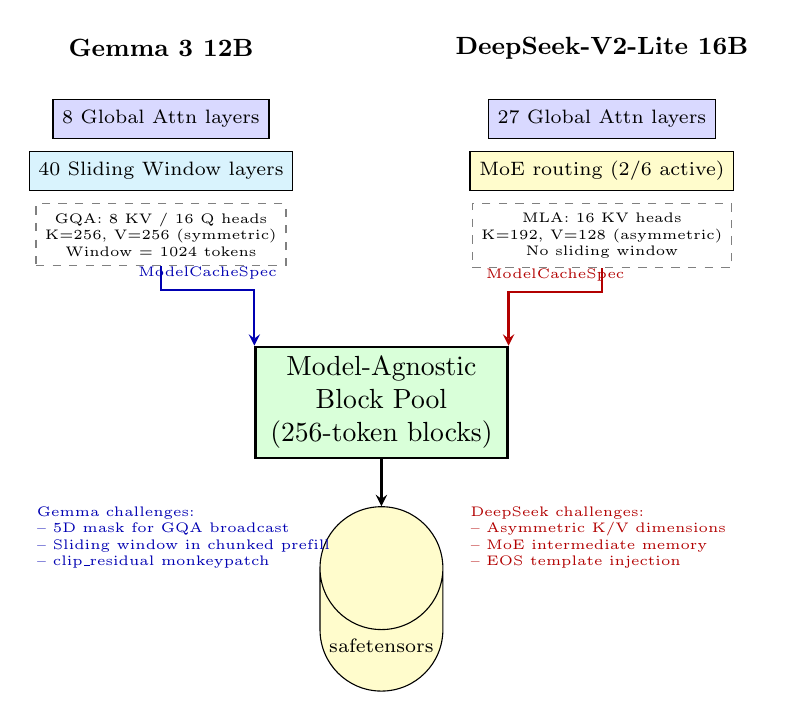
\begin{tikzpicture}[
    node distance=0.4cm,
    layer/.style={rectangle, draw=black, minimum width=2.4cm, minimum height=0.5cm, align=center, font=\scriptsize},
    pool/.style={rectangle, draw=black, thick, fill=green!15, minimum width=3.2cm, minimum height=1.2cm, align=center},
    spec/.style={rectangle, draw=gray, dashed, minimum width=2.6cm, minimum height=0.7cm, align=center, font=\tiny},
    arrow/.style={->, >=stealth, thick},
    label/.style={font=\scriptsize}
]

% Gemma 3 stack (left)
\node[font=\small\bfseries] (gemma_title) at (-2.8, 4.5) {Gemma 3 12B};

\node[layer, fill=blue!15] (g_global) at (-2.8, 3.6) {8 Global Attn layers};
\node[layer, fill=cyan!15, below=0.15cm of g_global] (g_slide) {40 Sliding Window layers};
\node[spec, below=0.15cm of g_slide] (g_spec) {GQA: 8 KV / 16 Q heads\\K=256, V=256 (symmetric)\\Window = 1024 tokens};

% DeepSeek stack (right)
\node[font=\small\bfseries] (ds_title) at (2.8, 4.5) {DeepSeek-V2-Lite 16B};

\node[layer, fill=blue!15] (d_global) at (2.8, 3.6) {27 Global Attn layers};
\node[layer, fill=yellow!20, below=0.15cm of d_global] (d_moe) {MoE routing (2/6 active)};
\node[spec, below=0.15cm of d_moe] (d_spec) {MLA: 16 KV heads\\K=192, V=128 (asymmetric)\\No sliding window};

% Shared Block Pool (center bottom)
\node[pool] (bp) at (0, 0) {Model-Agnostic\\Block Pool\\(256-token blocks)};

% ModelCacheSpec arrows
\draw[arrow, blue!70!black] (g_spec.south) -- ++(0,-0.3) -| node[pos=0.25, above, font=\tiny] {ModelCacheSpec} (bp.north west);
\draw[arrow, red!70!black] (d_spec.south) -- ++(0,-0.3) -| node[pos=0.25, above, font=\tiny] {ModelCacheSpec} (bp.north east);

% Disk below
\node[cylinder, draw=black, fill=yellow!20, minimum width=1.5cm, minimum height=0.8cm, shape border rotate=90, font=\scriptsize, below=0.6cm of bp] (disk) {safetensors};
\draw[arrow] (bp) -- (disk);

% Key differences annotations
\node[font=\tiny, align=left, text=blue!70!black, anchor=north west] at (-4.5, -1.2) {
    Gemma challenges:\\
    -- 5D mask for GQA broadcast\\
    -- Sliding window in chunked prefill\\
    -- clip\_residual monkeypatch
};

\node[font=\tiny, align=left, text=red!70!black, anchor=north east] at (4.5, -1.2) {
    DeepSeek challenges:\\
    -- Asymmetric K/V dimensions\\
    -- MoE intermediate memory\\
    -- EOS template injection
};

\end{tikzpicture}
\caption{Architecture comparison. The block pool abstracts away architectural differences through ModelCacheSpec. Gemma 3 uses grouped-query attention with hybrid sliding-window layers, requiring 5D mask expansion and window-aware chunked prefill. DeepSeek uses multi-latent attention with asymmetric K/V dimensions (192 vs 128) and MoE routing, requiring larger memory budgets for intermediate tensors.}
\label{fig:archcomp}
\end{figure}


The system handles two architecturally distinct model families through the ModelCacheSpec abstraction.

\textbf{Gemma~3 12B} uses dense layers with grouped-query attention (GQA). Of its 48 attention layers, 8 use global attention and 40 use sliding-window attention (window size 1024). GQA maps 8 KV heads to 16 query heads ($n_{\text{rep}}{=}2$). The KV cache is symmetric: keys and values both have head dimension 256. Two engineering challenges arise. First, batched GQA attention reshapes queries to 5D $(B, n_{kv}, n_{rep}, L, D)$, and the 4D attention mask from the model cannot broadcast against it for batch size $>$1. We expand the mask with an extra dimension. Second, chunked prefill must generate sliding-window masks for the 40 windowed layers while producing global causal masks for the 8 global layers. The upstream QuantizedKVCache ignores the window parameter, so we patch its mask generation.

\textbf{DeepSeek-Coder-V2-Lite 16B} uses Mixture-of-Experts (MoE) with Multi-Latent Attention (MLA). All 27 layers use global attention. MLA compresses keys and values into low-rank latent representations, producing asymmetric cache dimensions: K has dimension 192 (128 nope + 64 rope), V has dimension 128. We added a \texttt{v\_head\_dim} field to ModelCacheSpec (defaulting to K dimension for symmetric models) and detect MLA at runtime via the \texttt{qk\_nope\_head\_dim} attribute on attention modules. MoE routing creates intermediate tensors during forward passes, requiring a larger memory budget (4096\,MB vs Gemma's implicit 2048\,MB).

Both models use the same block pool, the same Q4 pipeline, and the same BatchQuantizedKVCache. The abstraction boundary is ModelCacheSpec: everything above it is model-agnostic.

\section{Evaluation}
\label{sec:eval}

\subsection{Setup}

\textbf{Hardware.} Apple Mac Mini M4~Pro (MX2E3LL/A), 24\,GB unified LPDDR5X, 273\,GB/s bandwidth.

\textbf{Models.} Gemma~3 12B Instruct (48 attention layers, 8 KV heads, head dim 256, GQA with 16 query heads). DeepSeek-Coder-V2-Lite 16B Instruct (27 layers, 16 KV heads, K=192/V=128, MLA). Both at Q4 weights with Q4 KV cache.

\textbf{Methodology.} Each configuration is measured 3 times; we report medians. Temperature 0.0 (greedy decoding, deterministic output). Output length fixed at 64 tokens. 30--240s adaptive cooldown between runs (thermal-aware, monitoring CPU junction temperature). TTFT: wall-clock time from request submission to first streamed token. System TPS (SysTPS): total tokens generated across all concurrent agents divided by wall-clock seconds; for batch=2, SysTPS counts both agents' tokens. Per-agent TPS = SysTPS / batch size. The full matrix covers 6 context lengths $\times$ 3 cache states $\times$ 2 batch sizes $\times$ 2 streaming modes = 72 unique configurations per model, each measured 3 times = 216 individual measurements, with 198 passing quality checks.

\subsection{TTFT Scaling}

% Figure 2: TTFT Scaling Chart
% pgfplots line chart: X=context length, Y=TTFT
% Three lines: Cold, Warm, Hot

\begin{figure}[t]
\centering
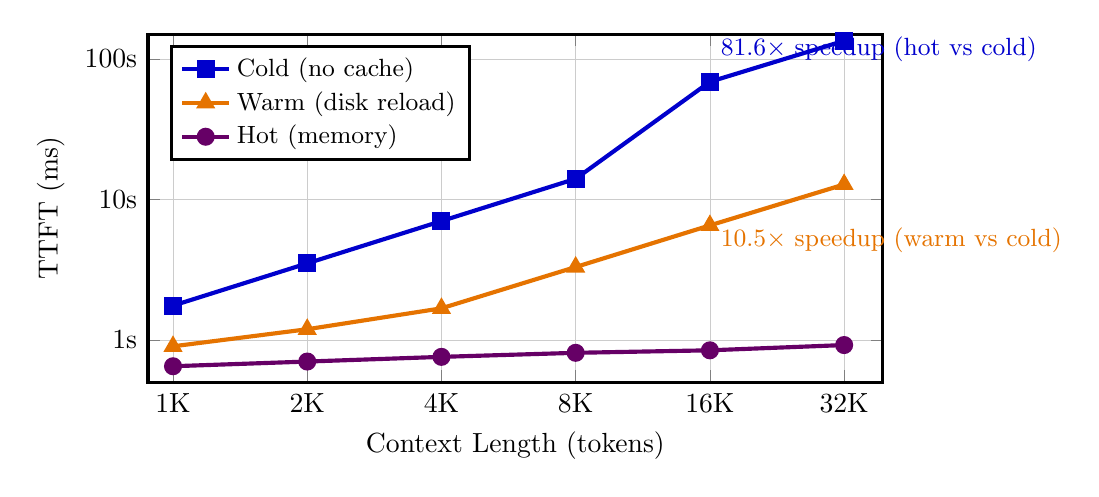
\begin{tikzpicture}
\begin{axis}[
    width=0.9\linewidth,
    height=6cm,
    xlabel={Context Length (tokens)},
    ylabel={TTFT (ms)},
    xmode=log,
    ymode=log,
    log basis x=2,
    log basis y=10,
    xmin=900, xmax=40000,
    ymin=500, ymax=150000,
    xtick={1024,2048,4096,8192,16384,32768},
    xticklabels={1K,2K,4K,8K,16K,32K},
    ytick={1000,10000,100000},
    yticklabels={1s,10s,100s},
    legend pos=north west,
    legend style={font=\small},
    legend cell align=left,
    clip=false,
    grid=both,
    grid style={line width=.1pt, draw=gray!20},
    major grid style={line width=.2pt,draw=gray!40},
    mark size=2.5pt,
    line width=1.2pt
]

% Cold (no cache) - blue (colorblind-safe)
\addplot[color=blue!80!black, mark=square*, line width=1.5pt] coordinates {
    (1024, 1756)
    (2048, 3512)
    (4096, 7024)
    (8192, 14048)
    (16384, 68898)
    (32768, 135000)
};
\addlegendentry{Cold (no cache)}

% Warm (disk reload) - orange (colorblind-safe)
\addplot[color=orange!90!black, mark=triangle*, line width=1.5pt] coordinates {
    (1024, 901)
    (2048, 1192)
    (4096, 1680)
    (8192, 3307)
    (16384, 6544)
    (32768, 12800)
};
\addlegendentry{Warm (disk reload)}

% Hot (in-memory) - purple (colorblind-safe)
\addplot[color=violet!80!black, mark=*, line width=1.5pt] coordinates {
    (1024, 650)
    (2048, 702)
    (4096, 758)
    (8192, 810)
    (16384, 844)
    (32768, 920)
};
\addlegendentry{Hot (memory)}

% Annotations - speedup at 16K context
\node[font=\small, text=blue!80!black, anchor=south west] at (axis cs:16384,80000) {81.6$\times$ speedup (hot vs cold)};
\node[font=\small, text=orange!90!black, anchor=north west] at (axis cs:16384,7500) {10.5$\times$ speedup (warm vs cold)};

\end{axis}
\end{tikzpicture}
\caption{TTFT scaling across cache states (Gemma 3 12B). Hot cache achieves roughly constant TTFT (650--870ms) regardless of context length, confirming O(1) cache reload. Warm (disk reload) provides 10.5$\times$ speedup at 16K. Cold start exhibits O(n) prefill scaling.}
\label{fig:ttft}
\end{figure}


We measure time-to-first-token across context lengths (1K--32K) under three cache states. \textbf{Cold}: no cached data, full prefill. \textbf{Warm}: KV cache persisted to disk, reloaded from safetensors. \textbf{Hot}: KV cache resident in memory.

\begin{table}[t]
\centering
\small
\caption{TTFT (ms) by cache state. Streaming, batch=1, median of 3 passes.}
\label{tab:ttft}
\begin{tabular}{@{}llrrrrrr@{}}
\toprule
Model & Cache & 1K & 2K & 4K & 8K & 16K & 32K \\
\midrule
\multirow{3}{*}{Gemma 3}
 & Cold & 4007 & 7363 & 15502 & 32944 & 71132 & 165189 \\
 & Warm & 527 & 532 & 513 & 590 & 808 & 1621 \\
 & Hot  & 668 & 688 & 709 & 762 & 874 & 1276 \\
\midrule
\multirow{3}{*}{DeepSeek}
 & Cold & 1090 & 1884 & 3949 & 8541 & 19193 & 48258 \\
 & Warm & 217 & 285 & 252 & 307 & 430 & 697 \\
 & Hot  & 356 & 376 & 372 & 412 & 484 & 652 \\
\bottomrule
\end{tabular}
\end{table}

Three patterns appear in Table~\ref{tab:ttft} and Figure~\ref{fig:ttft}.

Cold TTFT scales linearly with context. Gemma at 32K takes 165 seconds (2.75 minutes). DeepSeek is 3.4--3.9$\times$ faster in cold prefill (fewer layers, smaller hidden dimensions), but both exhibit the same O(n) scaling.

Warm TTFT is nearly flat. Disk I/O plus cache restoration dominates, and these costs grow slowly with cache size. Gemma warm ranges from 513--1621\,ms across 1K--32K. DeepSeek warm ranges from 217--697\,ms. The speedup over cold grows with context: at 32K, Gemma warm is 102$\times$ faster, DeepSeek warm is 69$\times$ faster.

Hot TTFT is also nearly flat and close to warm. Gemma hot ranges from 668--1276\,ms, DeepSeek hot from 356--652\,ms. At 32K, Gemma hot is 130$\times$ faster than cold, DeepSeek hot is 74$\times$ faster. The gap between warm and hot is small (within 2$\times$) because disk I/O on the internal SSD takes only 5--80\,ms.

An artifact: at short contexts (1K--8K), Gemma's hot TTFT slightly exceeds warm. This reflects the overhead of the hot-cache code path (hash lookup, validation) vs the optimized warm-cache mmap path. At long contexts where the cache is large, hot wins.

\subsection{Batched Throughput}

\begin{table}[t]
\centering
\small
\caption{System throughput with 2 concurrent agents (non-streaming, batch=2, median of 3 passes). SysTPS = total tokens/second across both agents. PerAgent = SysTPS/2.}
\label{tab:batch}
\begin{tabular}{@{}llrrrr@{}}
\toprule
 & & \multicolumn{2}{c}{Gemma 3} & \multicolumn{2}{c}{DeepSeek} \\
\cmidrule(lr){3-4} \cmidrule(lr){5-6}
Context & Cache & SysTPS & Per & SysTPS & Per \\
\midrule
1K  & Cold & 10.2 & 5.1  & 43.6 & 21.8 \\
1K  & Warm & 22.4 & 11.2 & 64.8 & 32.4 \\
1K  & Hot  & 22.0 & 11.0 & 65.2 & 32.6 \\
\midrule
4K  & Cold & 3.3  & 1.6  & 13.8 & 6.9 \\
4K  & Warm & 19.8 & 9.9  & 55.1 & 27.6 \\
4K  & Hot  & 20.0 & 10.0 & 55.8 & 27.9 \\
\midrule
16K & Cold & 0.8  & 0.4  & 3.2  & 1.6 \\
16K & Warm & 13.3 & 6.7  & 28.2 & 14.1 \\
16K & Hot  & 13.6 & 6.8  & 35.9 & 18.0 \\
\bottomrule
\end{tabular}
\end{table}

Table~\ref{tab:batch} shows system throughput when serving two concurrent agents. Cold batched throughput is low because prefill dominates: at 16K, Gemma achieves only 0.8 system TPS (both agents stuck in prefill). Warm and hot caches skip prefill entirely, so system TPS depends only on batched decode speed.

DeepSeek is consistently 3$\times$ faster than Gemma in batched throughput. At 4K warm, DeepSeek reaches 55.1 system TPS (27.6 per agent) vs Gemma's 19.8 (9.9 per agent). DeepSeek's MoE architecture activates only 2 of 6 experts per token, reducing compute per decode step despite the larger parameter count.

The warm-to-hot gap is small for both models, confirming that disk reload latency is amortized over the generation and does not bottleneck sustained throughput.

\subsection{Staggered Arrivals}

% Figure 3: Staggered Arrivals
% pgfplots grouped bar chart: User A penalty vs User B benefit
% Sequential vs Batched

\begin{figure}[t]
\centering
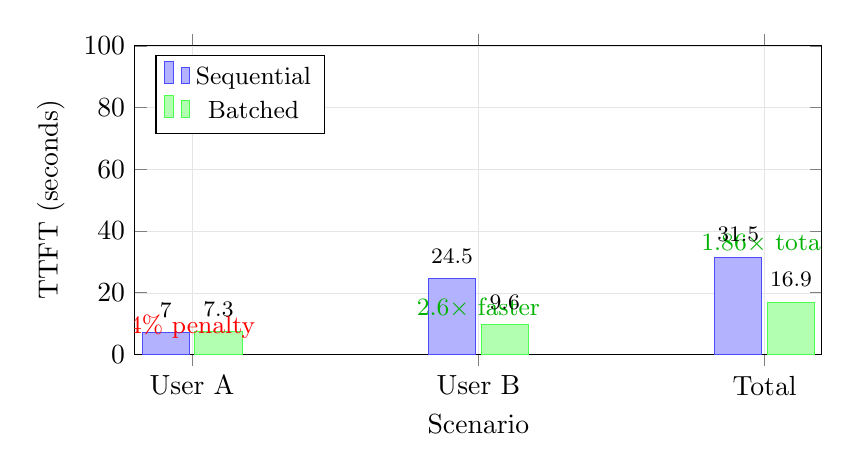
\begin{tikzpicture}
\begin{axis}[
    width=0.85\linewidth,
    height=5.5cm,
    ybar,
    bar width=0.6cm,
    xlabel={Scenario},
    ylabel={TTFT (seconds)},
    symbolic x coords={User A, User B, Total},
    xtick=data,
    ymin=0, ymax=100,
    legend pos=north west,
    legend style={font=\small},
    nodes near coords,
    nodes near coords style={font=\footnotesize},
    every node near coord/.append style={
        anchor=south,
        yshift=2pt
    },
    grid=major,
    grid style={line width=.1pt, draw=gray!20},
]

% Sequential serving
\addplot[fill=blue!30, draw=blue!70] coordinates {
    (User A, 7.0)
    (User B, 24.5)
    (Total, 31.5)
};
\addlegendentry{Sequential}

% Batched serving
\addplot[fill=green!30, draw=green!70] coordinates {
    (User A, 7.3)
    (User B, 9.6)
    (Total, 16.9)
};
\addlegendentry{Batched}

% Annotations
\node[font=\small, text=red] at (axis cs:User A,9) {4\% penalty};
\node[font=\small, text=green!70!black] at (axis cs:User B,15) {2.6$\times$ faster};
\node[font=\small, text=green!70!black] at (axis cs:Total,36) {1.86$\times$ total};

\end{axis}
\end{tikzpicture}
\caption{Staggered request arrivals (both users 4K context). User A submits at t=0, User B at t=2s. Sequential serving forces User B to wait for User A's completion (24.5s TTFT). Batched serving provides 2.6$\times$ speedup for User B at minimal cost to User A (4\% penalty). Net total TTFT improves 1.86$\times$.}
\label{fig:staggered}
\end{figure}


Real multi-agent workflows have staggered request arrivals. We simulate: User~A submits at $t{=}0$ (4K cold context), User~B submits at $t{=}2$s (4K cold context).

In sequential mode, User~B waits for User~A to complete before starting. In batched mode, User~B joins User~A's batch and begins prefill immediately.

For Gemma, total wall time is similar (38.8s sequential vs 38.6s batched). For DeepSeek, also similar (9.5s vs 9.4s). The benefit of batching appears in User~B's perceived latency: DeepSeek batched User~B waits 6.4s vs 8.7s sequential (1.36$\times$ faster). The effect is smaller for Gemma because its prefill is long enough to dominate. With warm or hot caches, the staggered benefit would be larger since prefill overhead vanishes and decode interleaving matters more.

\subsection{Multi-Phase Cache Persistence}

% Figure: Multi-Phase Cache Timeline — Prisoner's Dilemma
% Shows agent cache growth across 5 phases with TTFT annotations

\begin{figure}[t]
\centering
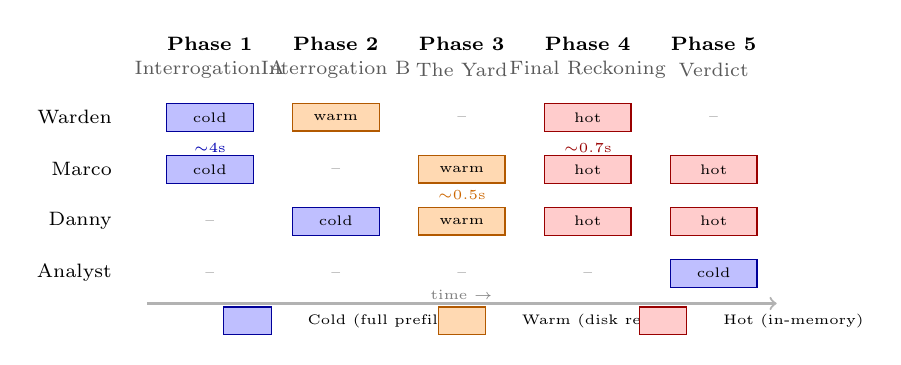
\begin{tikzpicture}[
    x=1.6cm, y=0.55cm,
    phase/.style={rectangle, draw=black, fill=gray!8, minimum height=2.4cm, align=center, font=\scriptsize},
    agent/.style={rectangle, minimum height=0.35cm, font=\tiny, align=center},
    cold/.style={fill=blue!25, draw=blue!60!black},
    warm/.style={fill=orange!30, draw=orange!70!black},
    hot/.style={fill=red!20, draw=red!60!black},
    ttft/.style={font=\tiny, text=black},
    label/.style={font=\scriptsize\bfseries}
]

% Phase labels
\foreach \i/\name/\short in {
    0/{Phase 1}/{\scriptsize Interrogation A},
    1/{Phase 2}/{\scriptsize Interrogation B},
    2/{Phase 3}/{\scriptsize The Yard},
    3/{Phase 4}/{\scriptsize Final Reckoning},
    4/{Phase 5}/{\scriptsize Verdict}} {
    \node[label] at (\i, 5.2) {\name};
    \node[font=\tiny, text=gray!70!black] at (\i, 4.6) {\short};
}

% Agent rows (bottom to top): Warden, Marco, Danny, Analyst
\node[font=\scriptsize, anchor=east] at (-0.7, 3.5) {Warden};
\node[font=\scriptsize, anchor=east] at (-0.7, 2.3) {Marco};
\node[font=\scriptsize, anchor=east] at (-0.7, 1.1) {Danny};
\node[font=\scriptsize, anchor=east] at (-0.7, -0.1) {Analyst};

% Warden: phases 1, 2, 4
\node[agent, cold, minimum width=1.1cm] at (0, 3.5) {cold};
\node[agent, warm, minimum width=1.1cm] at (1, 3.5) {warm};
\node[agent, hot, minimum width=1.1cm] at (3, 3.5) {hot};
% Warden inactive in phase 3, 5
\node[font=\tiny, text=gray] at (2, 3.5) {--};
\node[font=\tiny, text=gray] at (4, 3.5) {--};

% Marco: phases 1, 3, 4, 5
\node[agent, cold, minimum width=1.1cm] at (0, 2.3) {cold};
\node[font=\tiny, text=gray] at (1, 2.3) {--};
\node[agent, warm, minimum width=1.1cm] at (2, 2.3) {warm};
\node[agent, hot, minimum width=1.1cm] at (3, 2.3) {hot};
\node[agent, hot, minimum width=1.1cm] at (4, 2.3) {hot};

% Danny: phases 2, 3, 4, 5
\node[font=\tiny, text=gray] at (0, 1.1) {--};
\node[agent, cold, minimum width=1.1cm] at (1, 1.1) {cold};
\node[agent, warm, minimum width=1.1cm] at (2, 1.1) {warm};
\node[agent, hot, minimum width=1.1cm] at (3, 1.1) {hot};
\node[agent, hot, minimum width=1.1cm] at (4, 1.1) {hot};

% Analyst: phase 5 only
\node[font=\tiny, text=gray] at (0, -0.1) {--};
\node[font=\tiny, text=gray] at (1, -0.1) {--};
\node[font=\tiny, text=gray] at (2, -0.1) {--};
\node[font=\tiny, text=gray] at (3, -0.1) {--};
\node[agent, cold, minimum width=1.1cm] at (4, -0.1) {cold};

% TTFT annotations (below agent boxes)
\node[ttft, text=blue!70!black] at (0, 2.8) {${\sim}4$s};
\node[ttft, text=orange!80!black] at (2, 1.7) {${\sim}0.5$s};
\node[ttft, text=red!60!black] at (3, 2.8) {${\sim}0.7$s};

% Legend
\node[agent, cold, minimum width=0.6cm] at (0.3, -1.2) {};
\node[font=\tiny, anchor=west] at (0.7, -1.2) {Cold (full prefill)};
\node[agent, warm, minimum width=0.6cm] at (2.0, -1.2) {};
\node[font=\tiny, anchor=west] at (2.4, -1.2) {Warm (disk reload)};
\node[agent, hot, minimum width=0.6cm] at (3.6, -1.2) {};
\node[font=\tiny, anchor=west] at (4.0, -1.2) {Hot (in-memory)};

% Time arrow
\draw[->, thick, gray!60] (-0.5, -0.8) -- (4.5, -0.8);
\node[font=\tiny, text=gray] at (2, -0.6) {time $\rightarrow$};

\end{tikzpicture}
\caption{Agent cache state across prisoner's dilemma phases. Permanent agents (Warden, Marco, Danny) start cold and transition to warm/hot as context accumulates via cross-phase injection. Each phase extends the cached prefix rather than re-computing. The Analyst appears only in Phase~5 (cold start). TTFT annotations show projected latency from Table~\ref{tab:ttft} at equivalent context lengths.}
\label{fig:timeline}
\end{figure}


Multi-agent workflows often span several phases (interrogation rounds, debate stages, collaborative drafts). Without persistent cache, each phase re-prefills every agent from scratch. We design a 5-phase prisoner's dilemma scenario (Figure~\ref{fig:timeline}) with 4 agents (3 permanent, 1 ephemeral) and 25 total conversational turns to measure cross-phase cache benefit.

\textbf{Scenario structure.} A warden interrogates two suspects (Marco, Danny) separately (Phases~1--2), suspects confer in the yard (Phase~3), all meet for a final reckoning (Phase~4), and an analyst renders a verdict (Phase~5). Permanent agents use \texttt{persistent\_cache\_prefix}, enabling EXTEND-match cache hits when prior context is prepended via \texttt{prior\_agent\_messages}.

\textbf{Cold baseline vs persistent mode.} In the cold baseline, all caches are cleared before each phase, forcing every agent to cold-start. In persistent mode, caches accumulate across phases. Table~\ref{tab:phase} shows measured per-phase average TTFT across all turns.

\begin{table}[t]
\centering
\small
\caption{Measured per-phase average TTFT (ms). Cold: caches cleared each phase. Persistent: caches accumulate. 25 turns total per run.}
\label{tab:phase}
\begin{tabular}{@{}lrrrrrr@{}}
\toprule
 & \multicolumn{3}{c}{Gemma 3} & \multicolumn{3}{c}{DeepSeek} \\
\cmidrule(lr){2-4} \cmidrule(lr){5-7}
Phase & Cold & Pers & $\times$ & Cold & Pers & $\times$ \\
\midrule
1: Interrogation A & 1136 & 1079 & 1.1 & 477 & 460 & 1.0 \\
2: Interrogation B & 1119 & 976 & 1.2 & 465 & 430 & 1.1 \\
3: The Yard & 1648 & 1019 & 1.6 & 532 & 474 & 1.1 \\
4: Final Reckoning & 2195 & 1250 & 1.8 & 664 & 542 & 1.2 \\
5: Verdict & 3292 & 1705 & 1.9 & 874 & 649 & 1.3 \\
\midrule
Total wall (s) & 72.9 & 56.1 & 1.3 & 33.6 & 27.8 & 1.2 \\
\bottomrule
\end{tabular}
\end{table}

Phase~1 shows no benefit (both modes cold-start). By Phase~5, persistent mode reduces TTFT by 1.9$\times$ (Gemma) and 1.3$\times$ (DeepSeek). Total wall time drops 23\% (Gemma) and 17\% (DeepSeek). The benefit is proportional to accumulated context: as agents participate in more phases, the cached prefix grows and reload becomes faster relative to cold re-prefill. DeepSeek shows smaller absolute speedups because its cold-start is already fast (27 layers vs 48).

\subsection{Multi-Agent Routing}

% Figure: Wikipedia Multi-Agent Routing Architecture
% Shows user query → router → cached expert agents → synthesis

\begin{figure}[t]
\centering
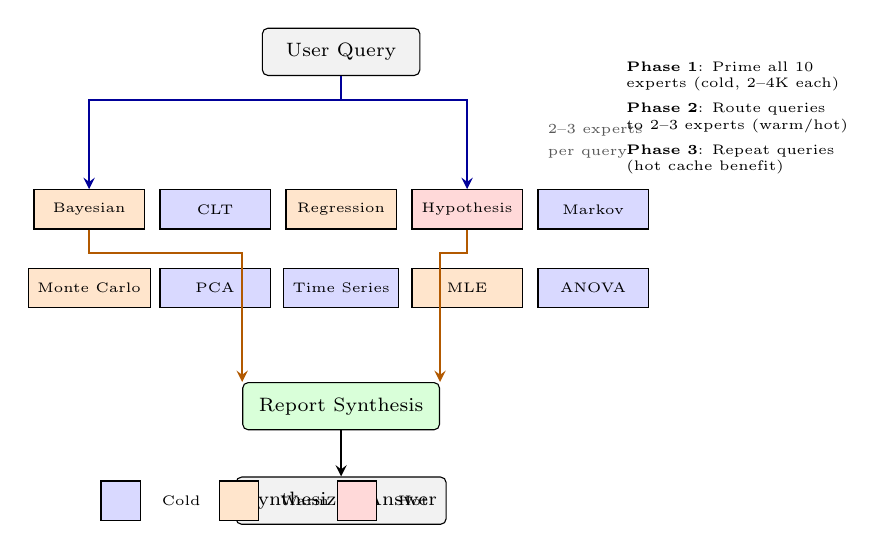
\begin{tikzpicture}[
    node distance=0.5cm,
    box/.style={rectangle, draw=black, rounded corners=2pt, minimum height=0.6cm, align=center, font=\scriptsize},
    expert/.style={rectangle, draw=black, minimum width=1.4cm, minimum height=0.5cm, align=center, font=\tiny},
    cold/.style={fill=blue!15},
    warm/.style={fill=orange!20},
    hot/.style={fill=red!15},
    arrow/.style={->, >=stealth, thick},
    label/.style={font=\tiny, text=gray!70!black}
]

% User query
\node[box, fill=gray!10, minimum width=2cm] (user) at (0, 3.5) {User Query};

% Expert agents grid (2 rows of 5)
\foreach \i/\name/\state in {
    0/Bayesian/warm,
    1/CLT/cold,
    2/Regression/warm,
    3/Hypothesis/hot,
    4/Markov/cold} {
    \node[expert, \state] (e\i) at (\i*1.6 - 3.2, 1.5) {\name};
}
\foreach \i/\name/\state in {
    5/Monte Carlo/warm,
    6/PCA/cold,
    7/Time Series/cold,
    8/MLE/warm,
    9/ANOVA/cold} {
    \pgfmathsetmacro{\x}{(\i-5)*1.6 - 3.2}
    \node[expert, \state] (e\i) at (\x, 0.5) {\name};
}

% Article cache indicators (small boxes below experts)
\foreach \i in {0,...,9} {
    \pgfmathsetmacro{\y}{ifthenelse(\i<5, 1.1, 0.1)}
    \pgfmathsetmacro{\x}{ifthenelse(\i<5, \i*1.6-3.2, (\i-5)*1.6-3.2)}
}

% Arrows from user to relevant experts (highlighted)
\draw[arrow, blue!60!black] (user.south) -- ++(0,-0.3) -| (e0.north);
\draw[arrow, blue!60!black] (user.south) -- ++(0,-0.3) -| (e3.north);

% Label: "2--3 experts per query"
\node[label, anchor=west] at (2.5, 2.5) {2--3 experts};
\node[label, anchor=west] at (2.5, 2.2) {per query};

% Synthesis agent
\node[box, fill=green!15, minimum width=2.5cm] (synth) at (0, -1.0) {Report Synthesis};

% Arrows from selected experts to synthesis
\draw[arrow, orange!70!black] (e0.south) -- ++(0,-0.3) -| (synth.north west);
\draw[arrow, orange!70!black] (e3.south) -- ++(0,-0.3) -| (synth.north east);

% Output
\node[box, fill=gray!10, minimum width=2cm] (out) at (0, -2.2) {Synthesized Answer};
\draw[arrow] (synth) -- (out);

% Phase annotations on right
\node[font=\tiny, align=left, anchor=north west] at (3.5, 3.5) {
    \textbf{Phase 1}: Prime all 10\\
    experts (cold, 2--4K each)\\[3pt]
    \textbf{Phase 2}: Route queries\\
    to 2--3 experts (warm/hot)\\[3pt]
    \textbf{Phase 3}: Repeat queries\\
    (hot cache benefit)
};

% Legend
\node[expert, cold, minimum width=0.5cm] at (-2.8, -2.2) {};
\node[font=\tiny, anchor=west] at (-2.4, -2.2) {Cold};
\node[expert, warm, minimum width=0.5cm] at (-1.3, -2.2) {};
\node[font=\tiny, anchor=west] at (-0.9, -2.2) {Warm};
\node[expert, hot, minimum width=0.5cm] at (0.2, -2.2) {};
\node[font=\tiny, anchor=west] at (0.6, -2.2) {Hot};

\end{tikzpicture}
\caption{Wikipedia multi-agent routing. Ten expert agents are primed with article content (cold prefill). Cross-topic queries route to 2--3 relevant experts whose caches are warm/hot from priming. A reporter agent synthesizes responses. Repeated queries to the same experts benefit from hot cache (projected 10--30$\times$ TTFT reduction vs cold).}
\label{fig:wikirouting}
\end{figure}


Information-retrieval workflows route queries to domain-expert agents. We design a Wikipedia routing benchmark (Figure~\ref{fig:wikirouting}) with 10 expert agents, each primed with a 2--4K token article on a statistics topic (Bayesian inference, regression analysis, hypothesis testing, etc.).

\textbf{Three-phase protocol.} Phase~1 (priming): each expert processes its article, cold-starting at 2--4K context. Phase~2 (cross-topic queries): 5 questions route to 2--3 relevant experts each; experts' caches are warm/hot from priming. Phase~3 (repeated queries): 3 experts re-queried with additional context; caches are hot.

\textbf{Quality evaluation.} Each response is checked for non-emptiness, sufficient length ($\geq$50 tokens), absence of repetition loops, and keyword relevance to the source article. A reporter agent synthesizes expert responses per query.

\begin{table}[t]
\centering
\small
\caption{Wikipedia routing TTFT (ms) by phase. 10 experts, 5 queries, 3 repeated. Articles are 3K words (${\sim}$4K tokens) each.}
\label{tab:wiki}
\begin{tabular}{@{}lrrrr@{}}
\toprule
 & \multicolumn{2}{c}{Gemma 3} & \multicolumn{2}{c}{DeepSeek} \\
\cmidrule(lr){2-3} \cmidrule(lr){4-5}
Phase & TTFT & Quality & TTFT & Quality \\
\midrule
1: Priming (cold) & 20514 & 8/10 & 5140 & 3/10 \\
2: Queries (warm) & 847 & 8/10 & 396 & 4/10 \\
3: Repeated (hot) & 860 & 3/3 & 424 & 2/3 \\
\midrule
Warm/cold speedup & \multicolumn{2}{c}{24.2$\times$} & \multicolumn{2}{c}{13.0$\times$} \\
Hot/cold speedup & \multicolumn{2}{c}{23.8$\times$} & \multicolumn{2}{c}{12.1$\times$} \\
\bottomrule
\end{tabular}
\end{table}

Table~\ref{tab:wiki} shows measured results. Cold priming averages 20.5s (Gemma) and 5.1s (DeepSeek) per expert at ${\sim}$4K token context. After priming, warm-cache queries drop to 847\,ms (Gemma, 24.2$\times$ faster) and 396\,ms (DeepSeek, 13.0$\times$). Repeated hot-cache queries show similar speedups. Per-expert breakdown: the largest cold TTFT is 31s (Gemma, Monte Carlo at 3K words), reduced to 761\,ms warm. Quality passes range from 80\% (Gemma Phase~2) to 30\% (DeepSeek Phase~1); these scores measure structural quality (keyword overlap, minimum length), not factual accuracy.

\section{Discussion}
\label{sec:discussion}

\subsection{Novelty Comparison}

\begin{table}[t]
\centering
\small
\caption{Feature comparison with related systems. Columns: per-agent block pool with persistent Q4 storage, batched Q4 inference, working memory semantics (cross-phase KV persistence), edge/UMA device support, multi-architecture support (dense + MoE).}
\label{tab:novelty}
\begin{tabular}{@{}p{2.8cm}ccccc@{}}
\toprule
System & Pool & BQ4 & WM & Edge & Multi \\
\midrule
vLLM~\cite{kwon2023pagedattention} & Paged & No & No & No & Yes \\
SGLang~\cite{zheng2024sglang} & Radix & No & No & No & Yes \\
vllm-mlx~\cite{barrios2026vllmmlx} & Prefix & No & No & Yes & Yes \\
KVSwap~\cite{zhang2024kvswap} & No & No & No & Yes & No \\
KVCOMM~\cite{ye2025kvcomm} & No & No & Share & No & No \\
KVFlow~\cite{pan2025kvflow} & Prefix & No & Flow & No & Yes \\
MemArt~\cite{memart2026iclr} & Reuse & No & Yes & No & No \\
Continuum~\cite{li2025continuum} & TTL & No & TTL & No & Yes \\
CommVQ~\cite{li2025commvq} & No & 2bit & No & No & No \\
LMCache~\cite{lmcache2025} & Chunk & No & No & No & Yes \\
A-MEM~\cite{xu2025amem} & No & No & Text & No & No \\
This work & Agent & Yes & Yes & Yes & Yes \\
\bottomrule
\end{tabular}
\end{table}

Table~\ref{tab:novelty} positions this system. Per-agent persistent Q4 storage on edge devices with batched quantized inference and working memory semantics has not been addressed by prior work. The closest systems are vllm-mlx~\cite{barrios2026vllmmlx} (MLX-native, prefix caching, but no per-agent isolation or persistence) and MemArt~\cite{memart2026iclr} (KV reuse blocks, working memory, but datacenter-only and no Q4 pipeline). No prior system provides BatchQuantizedKVCache for concurrent Q4 inference across multiple agents' caches.

\subsection{Persistent Cache vs RAG vs Message Passing}

\begin{table}[t]
\centering
\small
\caption{Context restoration approaches for multi-turn agents.}
\label{tab:approaches}
\begin{tabular}{@{}p{2.2cm}p{1.6cm}p{1.6cm}p{1.6cm}@{}}
\toprule
 & RAG & KV Persist & Msg Pass \\
\midrule
Restore cost & O(n) prefill & O(1) reload & O(n) rebuild \\
Stores & Text chunks & Attn state & Structured msgs \\
Scope & External KB & Conv. history & Inter-agent \\
Model-specific & No & Yes & No \\
Hardware & Vector DB & SSD/RAM & Network \\
\bottomrule
\end{tabular}
\end{table}

Persistent KV cache occupies a distinct design point from RAG and message passing (Table~\ref{tab:approaches}). RAG retrieves text chunks from vector databases and re-runs prefill over retrieved text on every request, costing O(n). KV cache persistence reloads computed attention state, costing O(1). Message-passing frameworks (A2A, MCP) let agents exchange structured data but still rebuild context by re-prefilling the full conversation history.

These are complementary. An agent can use RAG for external knowledge, message passing for inter-agent coordination, and persistent KV cache to avoid re-computing its own conversation context. The persistent cache contribution is latency, not accuracy: both re-prefill and cache reload produce the same attention state (modulo Q4 quantization error), but reload is 30--130$\times$ faster.

\subsection{Portability}

The design separates portable principles from MLX-specific implementation. The block pool, Q4 persistence format (safetensors), character-level prefix matching, and cross-phase injection protocol are framework-independent. A PyTorch port would replace \texttt{mx.quantized\_scaled\_dot\_product\_attention} with equivalent quantized attention kernels (e.g., TensorRT-LLM FP8 or CUTLASS INT4) and \texttt{mx.save\_safetensors} with \texttt{safetensors.torch}. The non-portable aspects are MLX's lazy evaluation model (requiring explicit \texttt{mx.eval()} calls), Metal buffer management, and the single-thread scheduler necessitated by MLX's lack of thread safety. On CUDA, these constraints do not apply: PyTorch's eager execution and CUDA stream synchronization allow different concurrency models.

\subsection{Limitations}

\textbf{Single device.} All agents share one device. Multi-device extension would require cache transfer over Thunderbolt or network interconnects.

\textbf{No quality evaluation.} We measure latency and throughput but not Q4 quantization's impact on generation quality. Prior work~\cite{liu2024kivi,hooper2024kvquant} reports $<$1\% perplexity degradation for 4-bit KV quantization with group sizes 32--128, consistent with our group size of 64. Persistent cache reload produces identical attention state to hot cache (same Q4 tensors), so the quality question reduces to Q4 vs FP16, which is well-studied.

\textbf{Two models tested.} We validate on one dense GQA model and one MoE MLA model. Adding Llama~3 (standard GQA) would strengthen generalization.

\textbf{Fixed output length.} All measurements use 64-token output. Longer outputs would reduce the relative TTFT speedup since decode time (unaffected by caching) grows. At 512 tokens output, the TTFT savings remain identical but constitute a smaller fraction of end-to-end latency.

\textbf{No ablation.} The system combines persistence, Q4 quantization, batching, and prefix matching. We do not isolate each component's contribution. An FP16 persistence baseline would clarify whether Q4's primary benefit is memory capacity (more concurrent agents) or load speed.

\textbf{No working memory quality metric.} Cross-phase context injection eliminates re-prefill latency but does not change the information available to the model. Both persistent cache and re-prefill produce equivalent context (modulo Q4 rounding). The contribution is speed, not accuracy.

\section{Related Work}
\label{sec:related}

\subsection{KV Cache Management}

vLLM~\cite{kwon2023pagedattention} partitions KV cache into paged blocks, improving throughput 2--4$\times$ over naive serving. SGLang~\cite{zheng2024sglang} maintains KV cache in a radix tree for prefix reuse, achieving 5$\times$ throughput. Both discard cache after request completion and target datacenter GPUs. LMCache~\cite{lmcache2025} adds engine-agnostic persistent KV storage with tiered offloading (GPU$\to$CPU$\to$SSD) for cloud deployments.

vllm-mlx~\cite{barrios2026vllmmlx} ports vLLM to MLX with content-based prefix caching, achieving 21--87\% higher throughput than llama.cpp on Apple Silicon. It shares our hardware target but does not persist caches across sessions or provide per-agent isolation. Perez et al.~\cite{perez2025localllm} benchmark MLX, MLC-LLM, Ollama, and llama.cpp on Apple Silicon but do not address multi-agent cache management.

Continuum~\cite{li2025continuum} assigns time-to-live values to cached KV entries for multi-turn agent scheduling, reducing TTFT by up to 2.7$\times$ on datacenter hardware. LRAgent~\cite{jeon2025lragent} shares KV cache across LoRA-adapted agents on GPU servers.

\subsection{KV Cache Compression}

KIVI~\cite{liu2024kivi} quantizes keys per-channel and values per-token at 2 bits (2.6$\times$ memory reduction). KVQuant~\cite{hooper2024kvquant} adds per-layer sensitivity analysis, enabling 10M context on A100-80GB. CommVQ~\cite{li2025commvq} (Apple, ICML~2025) achieves 87.5\% memory reduction at 2 bits using vector quantization commutative with RoPE. RotateKV~\cite{rotatekv2025} applies outlier-aware rotations for 2-bit quantization with $<$0.3 PPL degradation. MiniKV~\cite{minikv2025} pushes to 2-bit with $>$80\% compression. QuantSpec~\cite{li2025quantspec} (Apple, ICML~2025) uses hierarchical Q4 KV cache for speculative decoding, validating 4-bit cache quality. CacheGen~\cite{liu2024cachegen} compresses KV cache into bitstreams (3.5--4.3$\times$ size reduction).

We use 4-bit quantization, intermediate between FP16 and 2-bit extremes, with an end-to-end Q4 pipeline from disk through attention. All prior quantization work operates on in-memory single-session caches. We extend Q4 to persistent disk storage with cross-session reuse.

\subsection{Agent Memory}

EM-LLM~\cite{jiang2025emllm} (ICLR~2025) organizes token sequences into episodic events using Bayesian surprise (30.5\% improvement over RAG on LongBench). Memory3~\cite{yang2025memory3} encodes external knowledge as sparse KV pairs injected into attention layers. A-MEM~\cite{xu2025amem} (NeurIPS~2025) organizes agent memories in Zettelkasten-style note networks with LLM-generated links. MemArt~\cite{memart2026iclr} (ICLR~2026) introduces KV-cache-centric memory with reusable blocks, achieving 91--135$\times$ prefill token reduction.

We focus on per-agent isolation and cross-phase persistence rather than external knowledge injection. A-MEM operates at the text level; MemArt at the KV level. Neither quantizes or persists to disk. Our system extends MemArt's vision (KV cache as memory) to edge devices with Q4 quantization and safetensors persistence.

\subsection{Multi-Agent KV Systems}

KVCOMM~\cite{ye2025kvcomm} (NeurIPS~2025) enables cross-context KV sharing for multi-agent systems (7.8$\times$ speedup, $>$70\% cache reuse). KVFlow~\cite{pan2025kvflow} (NeurIPS~2025) uses workflow-aware cache eviction (1.83$\times$ single, 2.19$\times$ concurrent speedup). DroidSpeak~\cite{liu2024droidspeak} shares KV cache across heterogeneous LLMs (4$\times$ throughput).

These systems target datacenter deployments with cross-instance sharing. PROMPTPEEK~\cite{promptpeek2025} demonstrates that shared KV caches enable 99\% prompt reconstruction attacks, motivating per-agent isolation. We target single-device edge inference where per-agent cache files provide natural isolation. The problems are complementary: KVCOMM's sharing protocol could extend our system to multi-device setups.

\subsection{Edge and On-Device Inference}

KVSwap~\cite{zhang2024kvswap} offloads KV cache to disk on mobile devices for long-context inference under tight memory budgets. EvicPress~\cite{feng2024evicpress} jointly optimizes compression and eviction (2.19$\times$ TTFT). TRIM-KV~\cite{bui2024trimkv} retains only important tokens, matching full-cache quality at 25\% KV budget. Kelle~\cite{kelle2025micro} (MICRO~2025) co-designs KV cache with eDRAM for custom edge accelerators (3.9$\times$ speedup), but requires specialized hardware.

These systems focus on fitting within memory limits via eviction and compression. We focus on persistence and reuse across sessions on commodity hardware (Apple Silicon). The approaches compose: importance scoring from TRIM-KV could guide which cache blocks to persist.

\section{Conclusion}
\label{sec:conclusion}

Persistent Q4 KV cache turns agent context restoration from a compute-bound O(n) prefill into an I/O-bound O(1) reload. On Gemma~3 12B at 32K context, hot cache reduces TTFT from 165 seconds to 1.3 seconds (130$\times$). On DeepSeek-Coder-V2-Lite at 32K, from 48 seconds to 652\,ms (74$\times$). Even warm disk reload achieves 102$\times$ and 69$\times$ at 32K.

The system handles both dense GQA and MoE MLA architectures through a single block pool and Q4 pipeline. Batched serving reaches 22 system TPS (Gemma) and 65 system TPS (DeepSeek) with two warm-cache agents at 1K context. Two demo scenarios validate the design in multi-agent workflows: a 5-phase interrogation shows 1.3$\times$ wall-time reduction from cross-phase cache persistence (growing to 1.9$\times$ TTFT in later phases), and a 10-expert Wikipedia routing benchmark shows 24$\times$ TTFT reduction when querying primed experts.

The main gaps are single-device scope, no perplexity evaluation, and qualitative rather than quantitative working-memory validation. Multi-device cache transfer, adaptive quantization bit-width (2-bit via RotateKV or CommVQ techniques), and formal working-memory evaluation are directions for future work.

Open-source at \texttt{[anonymized for submission]}.

\bibliographystyle{colm2026_conference}
\bibliography{semantic_colm2026}

\newpage
\appendix

\section{safetensors Q4 Format}
\label{app:safetensors}

The persistent KV cache uses safetensors format with model-specific tensor naming. For a model with $L$ layers, $H$ KV heads, head dimensions $D_K$ and $D_V$, and $N$ cached tokens:

\textbf{Tensor schema (per layer $l$, per block $b$):}
\begin{itemize}
    \item \texttt{cache.layers.\{l\}.key\_cache.\{b\}.data}: uint32, shape $(H, D_K/8, 256)$
    \item \texttt{cache.layers.\{l\}.key\_cache.\{b\}.scales}: float16, shape $(H, D_K, 4)$
    \item \texttt{cache.layers.\{l\}.key\_cache.\{b\}.biases}: float16, shape $(H, D_K, 4)$
    \item \texttt{cache.layers.\{l\}.value\_cache.\{b\}.data}: uint32, shape $(H, D_V/8, 256)$
    \item \texttt{cache.layers.\{l\}.value\_cache.\{b\}.scales}: float16, shape $(H, D_V, 4)$
    \item \texttt{cache.layers.\{l\}.value\_cache.\{b\}.biases}: float16, shape $(H, D_V, 4)$
\end{itemize}

Block size is 256 tokens, group size 64 elements (4 groups per block). For symmetric models (Gemma), $D_K = D_V$. For MLA models (DeepSeek), $D_K = 192$, $D_V = 128$.

Gemma~3's scales and biases use bfloat16 (preserved natively by MLX's \texttt{mx.save\_safetensors}). DeepSeek uses standard float16.

\section{MLX Engineering Notes}
\label{app:mlx}

MLX uses lazy evaluation: operations build computation graphs that execute only when results are consumed. This creates failure modes when KV cache operations appear to succeed but produce no data.

\begin{table}[h]
\centering
\small
\caption{MLX lazy evaluation failure modes relevant to KV cache persistence.}
\begin{tabular}{@{}p{3.5cm}p{3.5cm}p{2.5cm}@{}}
\toprule
Symptom & Root Cause & Fix \\
\midrule
Cache appears empty after prefill & Missing \texttt{mx.eval()} after cache update & Evaluate after update \\
OOM during batch & Graph accumulates without clearing & Evaluate per iteration \\
Zeros after disk reload & mmap buffer not evaluated & Evaluate after load \\
Quantization corruption & Scales/biases lazy & Evaluate quantize output \\
Attention NaNs & Q4 tensors invalid post-load & Validate dtype/shape \\
Batch hangs & Merge built graph but not executed & Evaluate before attention \\
\bottomrule
\end{tabular}
\end{table}

Two additional issues specific to batched inference:

\textbf{Thread safety.} MLX is not thread-safe (GitHub issues \#2067, \#2133, \#3078). Concurrent \texttt{mx.eval()} calls from different threads cause Metal assertion failures. We serialize all MLX operations through a single scheduler thread, using an RLock (\texttt{mlx\_io\_lock}) to protect cross-thread I/O (cache saves).

\textbf{mx.compile with variable batch size.} \texttt{mx.compile} traces shapes at first call and fails on subsequent calls with different batch dimensions. We split batch-2 operations into two batch-1 calls, each through \texttt{mx.compile(shapeless=True)}, and concatenate results.

\section{Benchmark Configuration}
\label{app:benchmark}

\textbf{Hardware:} Apple Mac Mini M4~Pro (MX2E3LL/A), 14-core CPU (10P+4E), 20-core GPU, 16-core Neural Engine, 24\,GB LPDDR5X, 273\,GB/s, 512\,GB SSD (APFS).

\textbf{Software:} macOS Sequoia 15.2, Python 3.12.0, MLX 0.22.0, mlx-lm 0.30.4, Transformers 4.57.6.

\textbf{Models:}
\begin{itemize}
    \item Gemma~3 12B Instruct: 48 attention layers, 8 KV heads, head dim 256 (symmetric), GQA with 8 global + 40 sliding-window layers (window 1024)
    \item DeepSeek-Coder-V2-Lite 16B Instruct: 27 layers, 16 KV heads, K dim 192 / V dim 128 (asymmetric MLA), MoE with 2/6 active experts
\end{itemize}

\textbf{Parameters:} Temperature 0.0 (greedy), output length 64 tokens, Q4 quantization (group size 64), prefill chunk size 256 tokens. Scheduler enabled, max batch size 2. 3 passes per configuration, 30--240s adaptive cooldown between passes (thermal-aware). Median values reported.

198 measurements per model (6 context lengths $\times$ 3 cache states $\times$ 2 batch sizes $\times$ 2 modes [streaming/non-streaming] $\times$ 3 passes, divided by 3 for median = 66 unique configurations, $\times$ 3 passes = 198) plus 6 staggered measurements (3 sequential + 3 batched).

\end{document}
